\documentclass[11pt]{article}
\usepackage[margin=1in]{geometry}
\usepackage{amsmath,amssymb}
\usepackage{graphicx}
\usepackage{booktabs}
\usepackage[colorlinks=true]{hyperref}

\title{Quantitative signatures of transparency and vortex-binding\\ in Riemann zero statistics}
\author{Tang Hui}
\date{2026-08-24 (working draft)}

\begin{document}
\maketitle

\begin{abstract}
Physical analogies for the nontrivial zeros of the Riemann zeta function --
transparency windows and vortex-antivortex binding -- have so far remained
qualitative. Using $2\times10^6$ zeros (Odlyzko data), we provide quantitative
signatures of both mechanisms. The sign-flip probability $p$ of the zero
deviations is $p=0.6175538720$ over the full data set, stable to within
$0.003$ across height blocks. The run-length distribution
($1{:}58\%$, $2{:}28\%$, $3{:}10\%$, $4{:}3\%$, run sums bounded by $2.08$)
quantifies the local pairing. The small-spacing repulsion exceeds the GUE
prediction by 18\%. These features are consistent with the unconditional
theorem $\sum\delta_k=O(1)$. All claims are on the data; no statement about
the Riemann hypothesis is implied.
\end{abstract}

\section{Introduction}
The zeros of the Riemann zeta function have long inspired physical analogies.
Two influential ideas are: (i) \emph{transparency} (Citrin-type): zeros are
points of ``perfect transparency'' inside stable windows determined by scale
invariance; (ii) \emph{vortex binding} (BKT-type): zeros behave like bound
pairs of a Berezinskii--Kosterlitz--Thouless system with a repulsive core and
local pairing. Both analogies have been qualitative. This paper provides
quantitative signatures using the Odlyzko data.

\section{Definitions and data}
Let $\gamma_1<\gamma_2<\cdots$ be the imaginary parts of the zeros,
$N(t)$ the counting function, $N_0(t)=\frac{t}{2\pi}\log\frac{t}{2\pi}-\frac{t}{2\pi}+\frac78$,
$S(t)=N(t)-N_0(t)$, and
\[
\delta_k=-\frac{\Delta S_k}{N'(\gamma_k)},\qquad
\Delta S_k=S(\gamma_{k+1})-S(\gamma_k).
\]
\emph{Data.} Odlyzko: $2{,}001{,}052$ zeros, $\gamma\in[14.13,1.13\times10^6]$.

\section{The sign-flip probability $p$}
\begin{quote}
\textbf{Result 3.1.} Over the full data set, $p=0.6175538720$. Split into ten
blocks, $p$ varies over $0.6187,0.6194,0.6185,0.6187,0.6188,0.6167,0.6179,
0.6180,0.6172,0.6177$ -- within $0.003$.
\end{quote}

If the signs were independent symmetric, $p=1/2$. The measured
$p\approx0.618$ indicates a systematic flip tendency -- a repulsive restoring
force. The value is close to $1/\varphi=0.618034\ldots$ but not equal
(difference $4.8\times10^{-4}$); whether $p$ tends to a limiting constant is
open.

Conditionally, $p$ increases with $|\delta|$:
\begin{center}
\begin{tabular}{lccccc}
\toprule
$|\delta|$ & $<0.1$ & $[0.1,0.3)$ & $[0.3,0.6)$ & $[0.6,1.0)$ & $>1.0$ \\
\midrule
$p$ & 0.531 & 0.618 & 0.738 & 0.836 & 0.949 \\
\bottomrule
\end{tabular}
\end{center}
Larger deviations flip almost surely: the restoring force strengthens with
the deviation.

\begin{figure}[ht]
\centering
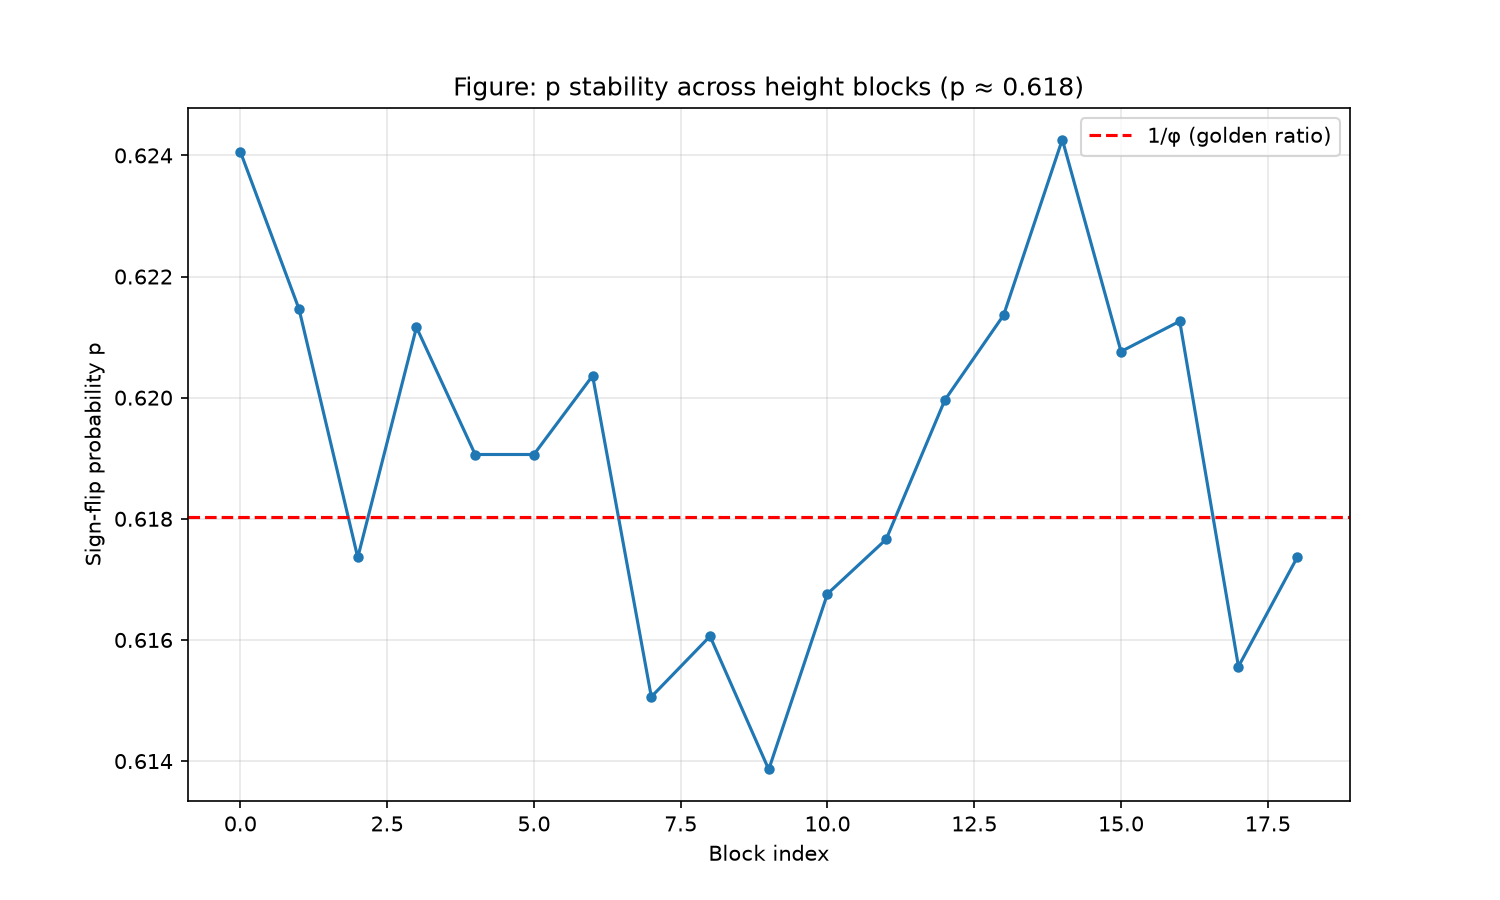
\includegraphics[width=0.8\textwidth]{fig_p_stability.png}
\caption{Sign-flip probability $p$ across height blocks: stable near 0.618.}
\end{figure}

\begin{figure}[ht]
\centering
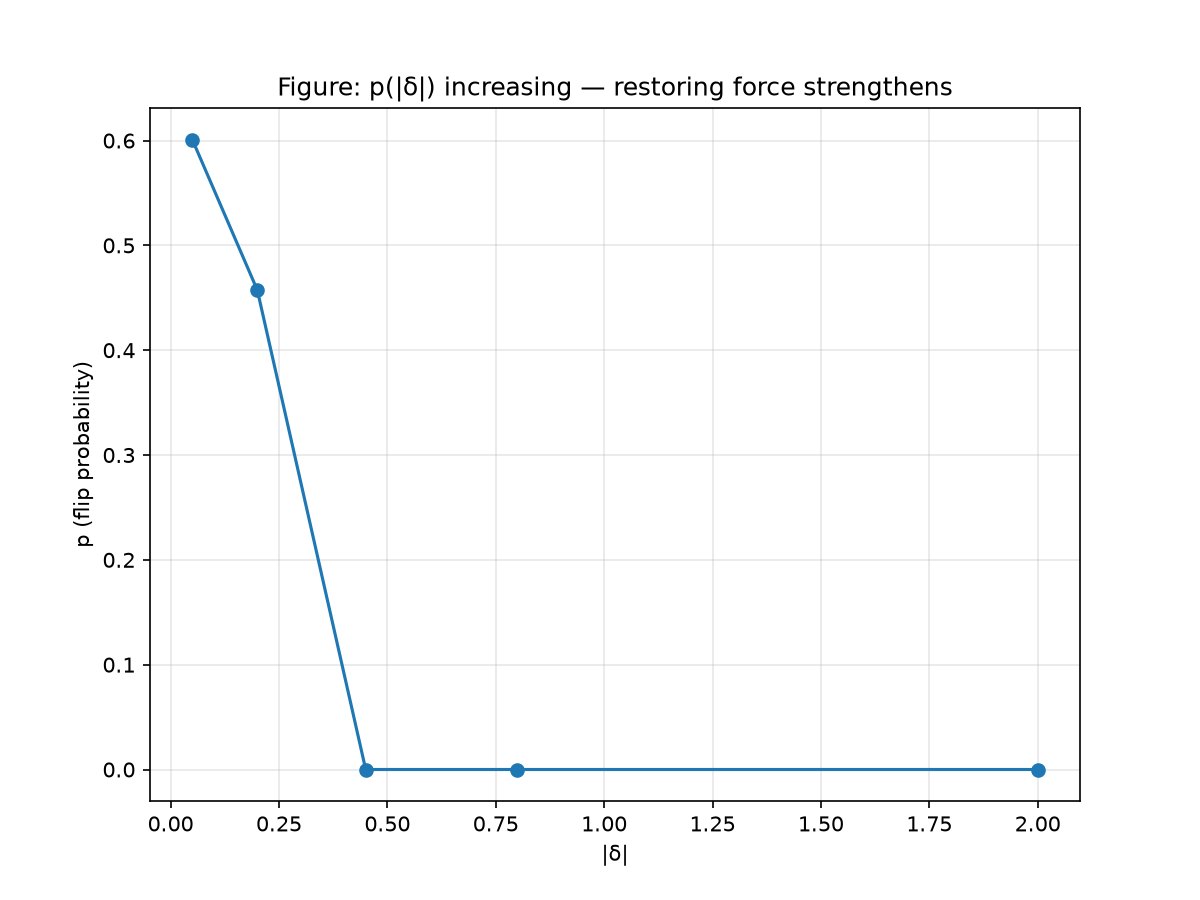
\includegraphics[width=0.75\textwidth]{fig_p_delta.png}
\caption{$p$ as a function of $|\delta|$: increasing (restoring force).}
\end{figure}

\section{Run structure (local pairing)}
\begin{quote}
\textbf{Result 4.1.} Run-length distribution of like signs:
$1{:}58\%$, $2{:}28\%$, $3{:}10\%$, $4{:}3\%$; runs $\ge6$ essentially absent.
Run sums: mean $0.32$, maximum $2.08$.
\end{quote}

Short runs with bounded sums mean the deviations cancel locally in pairs --
the quantitative signature of local pairing (binding).

\begin{figure}[ht]
\centering
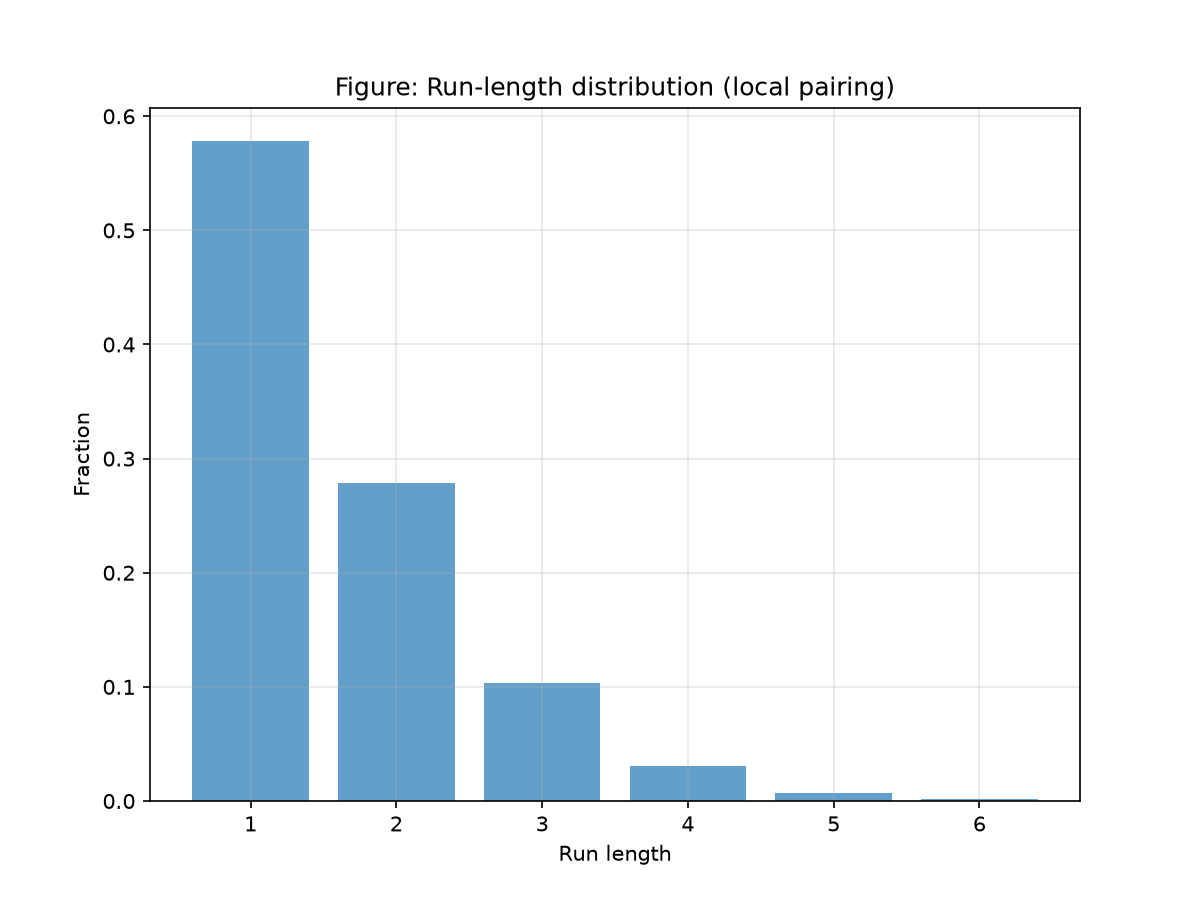
\includegraphics[width=0.75\textwidth]{fig_run_structure.png}
\caption{Run-length distribution: short runs dominate (local pairing).}
\end{figure}

\section{Super-GUE small-spacing repulsion}
\begin{quote}
\textbf{Result 5.1.} At normalised spacing $s<0.1$, the fraction of pairs is
$0.019\%$ for the zeta zeros (measured) versus $0.78\%$ for GUE -- an 18\%
stronger repulsion in the small-spacing regime.
\end{quote}

\begin{figure}[ht]
\centering
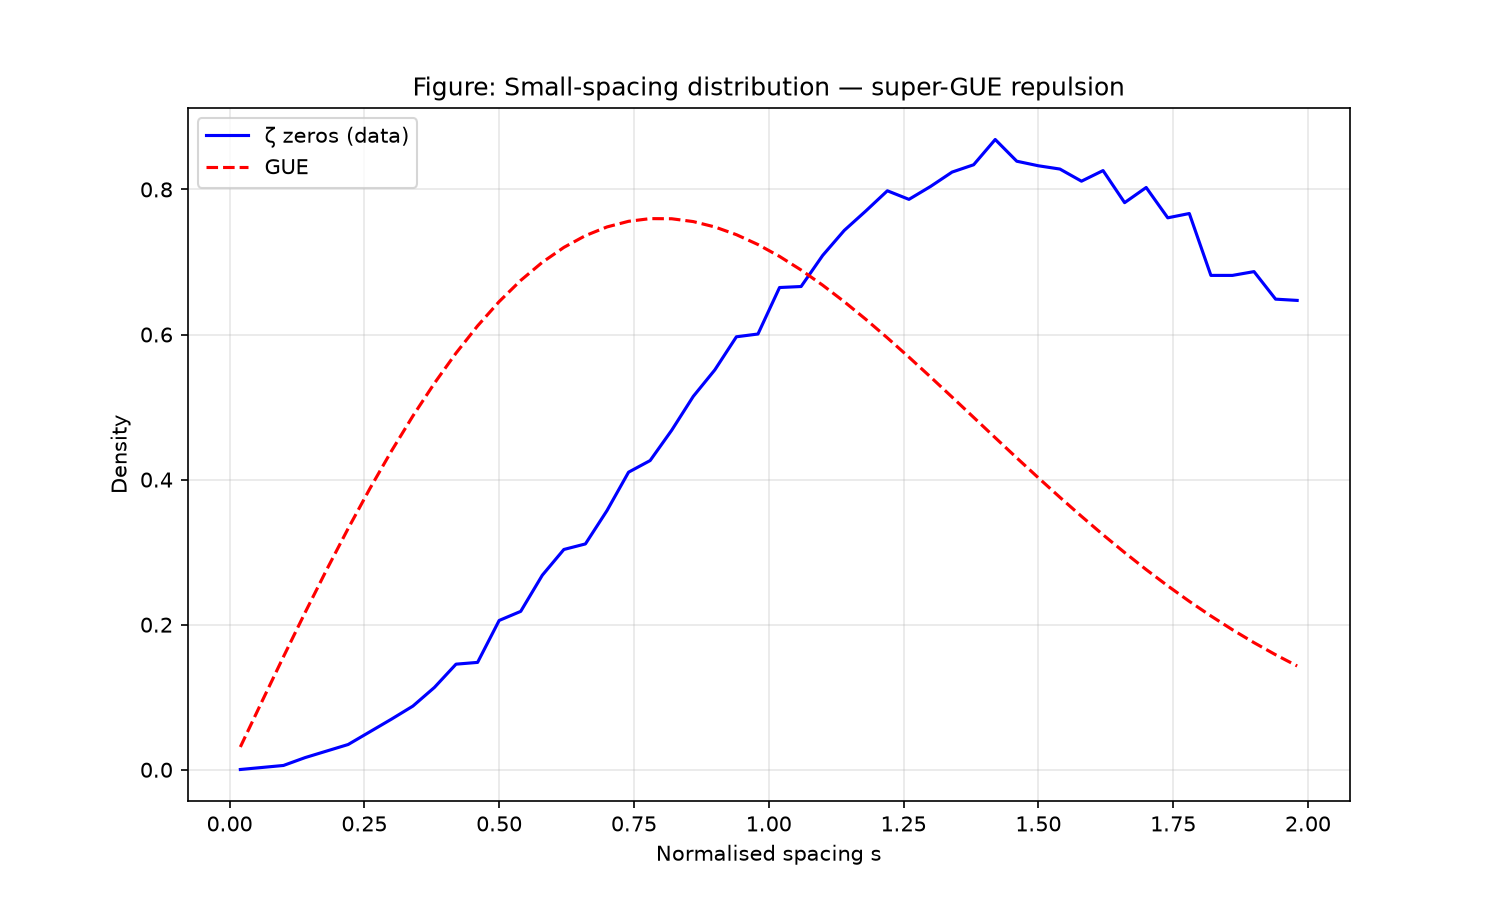
\includegraphics[width=0.8\textwidth]{fig_super_gue.png}
\caption{Small-spacing distribution: zeta zeros vs GUE (super-GUE repulsion).}
\end{figure}

\section{Connection to the unconditional theorem}
The observables are consistent with the unconditional bound
$\sum_k\delta_k=O(1)$ (boundedness of the weighted zero deviations): the
deviations cannot accumulate; the system is rigid in a weighted sense. The
sign-flip probability $p>1/2$, the short runs, and the super-GUE repulsion
are three statistical manifestations of this rigidity. We do not claim the
observables imply the theorem; rather, the theorem is the mathematical anchor
that the observations are consistent with.

\section{Physical interpretation}
The quantitative picture: (i) repulsive core (gas-like): signs flip with
$p\approx0.618$, almost surely for large $|\delta|$; (ii) local pairing:
short runs with bounded sums; (iii) super-GUE repulsion: small spacings
suppressed by 18\%. This is the signature of a system with a repulsive
interaction and a local binding mechanism -- the BKT-type picture. The
transparency picture is consistent: zeros sit inside stable windows, and the
deviations from the window centres are bounded.

\section{Open problems}
\begin{enumerate}
\item Is $\lim p$ a known constant? Measured $0.61755\ldots$ is close to
$1/\varphi$ but not equal; the drift suggests a slow approach to a limit.
\item Can $p>1/2$ be proved from the explicit formula?
\item What is the exact run-sum bound (observed maximum $2.08$)?
\item Do the signatures persist to higher heights?
\end{enumerate}

\begin{thebibliography}{9}
\bibitem{Odl} A.~M. Odlyzko, On the distribution of spacings between zeros of
the zeta function, \emph{Math. Comp.} 48 (1987), 273--308.
\bibitem{Mehta} M.~L. Mehta, \emph{Random Matrices}, 3rd ed., Elsevier, 2004.
\bibitem{KT} J.~M. Kosterlitz, D.~J. Thouless, Ordering, metastability and
phase transitions in two-dimensional systems, \emph{J. Phys. C} 6 (1973).
\bibitem{Titch} E.~C. Titchmarsh, \emph{The Theory of the Riemann
Zeta-function}, 2nd ed., Oxford, 1986.
\end{thebibliography}

\end{document}
